% !TEX root = main.tex
% !TEX program = pdflatex
% Revision 2026-09-20: C_two_papers/first_paper.md.
% Empirical source: Key_Experiment. Blank numeric cells mean unavailable evidence.
% Original manuscript/PDF preserved in revision_20260920/main.before.{tex,pdf}.
\pdfminorversion=7
\documentclass[final,5p,times,number]{elsarticle}
\usepackage{amsmath,amssymb,amsfonts}
\usepackage[ruled,vlined,linesnumbered]{algorithm2e}
\usepackage{graphicx,booktabs,tabularx,array,multirow}
\usepackage{xcolor,lmodern,microtype}
\usepackage{placeins}
\usepackage{tikz}
\usetikzlibrary{arrows.meta,positioning,fit,calc}
\usepackage[hidelinks]{hyperref}
\hypersetup{pdfauthor={Ketang Chen and Xiaolei Ren},
pdftitle={When Protocol States Mislead: Evidence-Gated Admission and Online Feedback Calibration for LLM-Assisted Stateful Fuzzing}}
\biboptions{sort&compress}
\journal{Journal of Network and Computer Applications}
\emergencystretch=2em
\newcommand{\missing}{\mbox{}}
\newcommand{\gcode}{G_{\mathrm{code}}}
\newcommand{\gstate}{G_{\mathrm{state}}}
\newcommand{\blankpanel}[1]{\fbox{\begin{minipage}[c][#1][c]{0.93\linewidth}\mbox{}\end{minipage}}}
\newcolumntype{Y}{>{\raggedright\arraybackslash}X}
\newcommand{\figref}[1]{Fig.~\ref{#1}}
\setlength{\tabcolsep}{4pt}
\begin{document}
\begin{frontmatter}
\title{When Protocol States Mislead: Evidence-Gated Admission and Online Feedback Calibration for LLM-Assisted Stateful Fuzzing}
\author[inst1]{Ketang Chen}
\ead{3250006913@student.must.edu.mo}
\author[inst1]{Xiaolei Ren\corref{cor1}}
\ead{xlren@must.edu.mo}
\cortext[cor1]{Corresponding author: Xiaolei Ren.}
\affiliation[inst1]{organization={Macau University of Science and Technology},
addressline={Avenida Wai Long, Taipa},city={Macau},country={China}}
\begin{abstract}
Response-derived states provide inexpensive scheduling feedback for network protocol fuzzing, but state-space expansion need not indicate progress through program code. Large language models (LLMs) introduce another source of uncertain proposals: a plausible request can consume long-term mutation resources without yielding useful executions. We present LoopFuzz as an evidence-calibration controller with two complementary mechanisms. Execute-before-promote admission separates structural validity, response acceptability, and state reachability from independent code and state novelty. Candidates with only state novelty receive bounded provisional validation; durable promotion requires code evidence. Online state-productivity calibration uses discounted Beta--Bernoulli updates at state-selection episodes and combines Thompson samples with frontier exploration. It estimates the usefulness of an observed state proxy, without attempting to recover semantic protocol states. We specify five experimental arms that separate admission from scheduling calibration under matched model policies and resource ceilings, together with information-controlled historical vulnerability rediscovery. The available nine-target archive contains AFLNet and recorded LoopFuzz runs, including interrupted runs, but does not yet establish either causal effect. We report recoverable evidence separately from the confirmatory protocol and leave unavailable results blank. Calibration, queue-pollution reduction, and vulnerability-rediscovery benefits remain to be tested.
\end{abstract}
\begin{keyword}
Stateful protocol fuzzing \sep Response-derived state feedback \sep Evidence-gated admission \sep Provisional queue \sep Online productivity calibration
\end{keyword}
\end{frontmatter}

\section{Introduction}
Stateful protocol fuzzing must discover useful interaction sequences as well as useful message contents. A server can accept a request only after earlier exchanges establish a session, authenticate a client, or create a resource. AFLNet uses responses to construct an inferred protocol state machine (IPSM), making protocol-visible feedback available without a target-specific internal-state extractor~\cite{aflnet}. This deployment advantage comes with an abstraction boundary: a response code or sequence is evidence about observable behavior, rather than an identifier of the server's complete semantic state.

StateAFL already identifies limitations of response-derived state abstractions and uses memory observations to infer server states~\cite{stateafl}. The fact that responses can misrepresent internal progress is therefore established background. Our question is how a fuzzer retaining a response-visible abstraction should decide, during a campaign, whether a particular state signal is useful enough to justify further exploration. A new IPSM state edge can accompany a previously unseen code branch, reproduce an already explored rejection path, or distinguish responses after the measured code surface has saturated. These outcomes should not receive identical evidential weight.

LLM-assisted protocol fuzzing makes this distinction consequential for queue management. ChatAFL demonstrates that language models can derive protocol structures and propose interaction sequences~\cite{chatafl}. A generated request is nevertheless a hypothesis about both message structure and live session conditions. If a proposal is retained indefinitely because it produces a new response-derived state, the fuzzer may repeatedly mutate an input whose apparent novelty has little downstream code value. Durable queue membership represents a continuing allocation of execution resources.

Three target families motivate the investigation. Forked-daapd exposes DAAP/DACP behavior through HTTP status responses, so response distinctions may overstate useful code progress. Lighttpd1 can execute different code paths under the same HTTP status, so response novelty may understate code progress. LightFTP motivates examining continuing IPSM growth after code-coverage saturation. These are hypotheses inherited from earlier development observations, not conclusions imposed on the present archive. Section~\ref{sec:motivation} separates them from the available measurements.

LoopFuzz addresses this problem through evidence-gated admission and online state-productivity calibration. It first checks a proposal's structure, then executes a bounded trial and separates response acceptability, state reachability, code novelty, and IPSM novelty. Code-supported candidates can enter the durable queue. State-only candidates receive a provisional validation budget and must earn durable promotion through subsequent code evidence. At the scheduling layer, a discounted productivity estimate conditions investment on the observed relationship between selected response states and later code progress.

This work makes three contributions, with their current evidence status stated explicitly.
\begin{enumerate}
\item \textbf{Evidence-gated queue admission.} We specify an execute-before-promote controller that distinguishes reject, provisional, and durable outcomes. It separates state novelty from code evidence and makes the lifetime and descendant cost of provisional entries auditable.
\item \textbf{Online calibration of state productivity.} We formulate response-state utility as the probability of code progress in a bounded state-selection episode. Discounted Beta--Bernoulli updates and Thompson sampling instantiate the controller; these established estimation and selection methods are not claimed as new algorithms.
\item \textbf{A controlled empirical framework with partial evidence.} We define candidate-level and episode-level measurements, five arms, launch accounting, and information-controlled rediscovery on vulnerable/patch-paired targets. We audit the supplied archive and identify the missing evidence for causal admission and calibration claims.
\end{enumerate}
The available evidence does not justify describing the third contribution as a completed five-arm evaluation. Preserving this distinction allows the design, implementation, and later experiments to be evaluated against the same explicit contract.

\section{Background and Motivation}
\label{sec:motivation}
\subsection{Response-visible state and independent code feedback}
Let $\mathcal{M}_t=(Q_t,\widehat{\Delta}_t,q_0)$ be the IPSM observed by time $t$, where $Q_t$ contains response-derived state identifiers, $\widehat{\Delta}_t\subseteq Q_t\times Q_t$ contains observed IPSM state edges, and $q_0$ denotes the initial connection state. The abstraction can alias different internal states and separate executions that reach the same code. It can also depend on history, asynchronous replies, and reset behavior. It is not assumed deterministic or semantically complete.

Let $\mathcal{B}_t$ be the covered code-branch set under a fixed instrumentation and replay pipeline. An IPSM state-edge increment changes $\widehat{\Delta}_t$; a code-branch increment changes $\mathcal{B}_t$. These objects have distinct units. An AFL bitmap observation must also distinguish a newly encountered code edge from a hit-count bucket change. Neither bitmap slots nor response-state identifiers are interchangeable with source-level code branches.

\subsection{Three falsifiable mismatch cases}
Table~\ref{tab:boundary} defines the three motivating cases; \figref{fig:mismatch} shows the corresponding observations available from the supplied archive. Establishing a mismatch mechanism requires comparable builds, a shared observation horizon, and execution-level or time-resolved evidence. Endpoint differences alone do not establish which state caused a difference. The partial archive must be allowed to contradict the earlier negative-target narrative.

\begin{table*}[t]
\centering\small
\caption{Motivating mismatch hypotheses and their present evidential boundary.}
\label{tab:boundary}
\begin{tabularx}{\textwidth}{l Y Y Y}
\toprule
Target & Hypothesis & Required observation & Current interpretation \\
\midrule
Forked-daapd & Overestimation: IPSM state-edge growth without downstream code gain. & Selected-state episodes with growing IPSM structure and low code reward. & The new archive does not reproduce the older endpoint code regression. \\
Lighttpd1 & Underestimation: code exploration within a shallow response abstraction. & Code-branch gain with little IPSM state-edge gain, joined to executions. & Both native endpoint metrics increase; their aggregate changes do not establish hidden productive states. \\
LightFTP & Saturation mismatch: response novelty persists after code progress plateaus. & Aligned code-branch and IPSM state-edge trajectories before and after saturation. & Near-equal native code endpoints motivate the test; current-build trajectories are still required. \\
\bottomrule
\end{tabularx}
\end{table*}

\begin{figure*}[t]
\centering\includegraphics[width=0.92\textwidth]{revision_20260920/native_endpoints.pdf}
\caption{Observed native terminal code-branch and IPSM state-edge counts for the three motivating targets (mean and sample standard deviation; ten supplied runs per target and label). All runs, including interruptions, are retained. Runtime and provenance differences prevent a matched-horizon causal interpretation. This figure tests the earlier narrative against current observations: it does not assert that all three hypothesized mismatch types were reproduced.}
\label{fig:mismatch}
\end{figure*}

The desired controller must accommodate both overestimation and underestimation. Rejecting every state-only candidate could lose useful bridges; promoting every such candidate would treat an imperfect proxy as sufficient evidence for permanent resource allocation. A provisional queue expresses the intermediate conclusion that an input deserves limited descendant validation while its longer-term value remains unproven.

The scope is textual or semi-textual request-response protocols with usable parsers, response extractors, and code feedback. Response-visible state extraction avoids a target-specific internal-state adapter, but the complete controller remains greybox because productivity requires code feedback. It is not a pure black-box system. Encrypted or opaque binary protocols require suitable construction, response, and code-observation adapters before evaluation.

\section{Related Work and Novelty Boundary}
Stateful greybox fuzzing studies how to expose, infer, and schedule protocol state~\cite{aflnet,stateafl,nsfuzz,sgf_usenix22}. AFLNet supplies a response-derived IPSM, whereas StateAFL and NSFuzz use different internal observations. LoopFuzz retains the response-visible interface and studies its instrumental reliability under an independent code-progress criterion. It does not claim to be the first system to identify state aliasing or misleading responses.

LLM-assisted generation addresses structured inputs and interaction histories~\cite{chatafl,fuzz4all_universal_fuzzing_large_2024,llmif_augmented_large_language_2024}. Grammar-aware and documentation-guided methods likewise improve input structure~\cite{gramatron_effective_grammar_aware_2021,carpetfuzz_documentation_2023}. Better proposals still need execution evidence before acquiring long-term queue resources. Our controlled ChatAFL comparison preserves its scheduling lineage rather than replacing its scheduler.

State and seed scheduling already use adaptive resource allocation. The Bandit's States studies bandit-based protocol-state selection; T-Scheduler applies Thompson-sampling ideas to fuzzing scheduling; SSGFuzz studies state significance in protocol fuzzing.\footnote{Reference completion required before submission: full bibliographic records for The Bandit's States, T-Scheduler, SSGFuzz, and Magma remain unverified. Their names and comparison roles are supplied by the revision brief; no author, year, venue, or DOI has been inferred.} These systems delimit the novelty claim: a bandit or productivity score is not itself a contribution. The distinction here is the combination of a response-derived proxy, an independent code-progress target, two-tier LLM-candidate admission, and auditable episode evidence.

Benchmark methodology requires repeated trials, comparable instrumentation, explicit budgets, and careful failure interpretation~\cite{profuzzbench_benchmark_stateful_protocol_2021,sok_prudent_evaluation_practices_2024,reliability_benchmarking_2022}. Historical vulnerability benchmarks such as Magma motivate distinguishing execution reaching bug-related code from execution satisfying a trigger condition. We adopt that distinction for network-reachable vulnerable/patch pairs; crash-file counts are not the unit of security success.
% Magma bibliographic record is pending as disclosed in the related-work footnote.

\begin{table*}[t]
\centering\small
\caption{Prior work and novelty boundary. This compares mechanisms, not measured performance.}
\label{tab:novelty}
\begin{tabularx}{\textwidth}{l Y Y}
\toprule
Prior work & Established focus & Present boundary \\
\midrule
AFLNet; StateAFL; NSFuzz & Response-derived or internal-state feedback. & Calibrate a retained response proxy without claiming semantic-state recovery. \\
ChatAFL; LLM synthesis & Protocol-informed message/sequence proposals. & Execute-before-promote and bounded provisional validation. \\
The Bandit's States & Bandit-based protocol-state selection. & Bandit formulation is prior art; independent reward and queue evidence are the focus. \\
T-Scheduler & Probabilistic adaptive fuzzing scheduling. & Beta estimation and Thompson sampling are reused components. \\
SSGFuzz & State-significance-guided protocol fuzzing. & Distinguish state importance from calibration against code productivity. \\
Magma; evaluation methodology & Ground-truth bug conditions and repeated evaluation. & Information-controlled network rediscovery with minimal security-patch pairs. \\
\bottomrule
\end{tabularx}
\end{table*}

\section{Evidence-Calibrated Controller}
\label{sec:design}
This section specifies the controller contract. Section~\ref{sec:implementation} identifies where the inspected implementation and archive do not yet satisfy it. A mathematical design rule is not evidence that a completed campaign obeyed that rule.

\subsection{LLM proposal interface}
The model receives permitted RFC fragments, seed traces, and observed interaction summaries and returns candidate requests or bounded scheduling hints. Each candidate has a persistent identifier, source state, intended target/frontier, and links to its prompt and raw reply. Message-field hypotheses remain proposals rather than verified protocol grammars.

The information policy excludes CVE identifiers, security advisories, exploit inputs, and patch contents. It fixes which documentation and live responses may be supplied. Identical information policy does not imply identical prompt bytes after adaptive campaigns diverge; prompt and reply hashes expose that distinction.

Request-producing outputs pass through admission. Scheduling-only outputs require schema, state-ID, and seed-ID checks and cannot insert durable inputs. Parsing or transport failure does not create a positive admission decision. All attempts, retries, failures, and successful replies enter the declared call/token accounting.

\subsection{Admission predicates and evidence separation}
For candidate $x$, $P(x)$ checks schema, message structure, required fields, lengths, and terminators before execution. A bounded trial then evaluates response acceptability $U(x)$ and reachability $R(x)$: arrival at a declared target/frontier or escape from a recorded rejection sink. Table~\ref{tab:predicates} gives operational evidence and required reason codes.

HTTP/FTP 4xx/5xx classes are rejection priors, not a universal semantic definition. An adapter must specify exceptions before a run and retain the response and reason code. Timeout, reset, disconnect, or an unparseable response gives no positive $U$ evidence. A valid response alone is insufficient for $R$. Security-oracle artifacts are retained independently even when normal request admission fails.

Gain is split into
\begin{align}
\gcode(x)&=\mathbf{1}\{\text{new code coverage or a favored}\nonumber\\
&\hspace{18mm}\text{code-coverage entry}\},\label{eq:gcode}\\
\gstate(x)&=\mathbf{1}\{\text{new IPSM node, state edge, or path}\}.\label{eq:gstate}
\end{align}
Favored status must be grounded in code coverage; merely being queued or state-novel does not qualify. Source-level code branches are the main evaluation surface. If runtime instrumentation observes code edges instead, that reward definition must be frozen and reported separately. Hit-count novelty is a separate sensitivity condition. Pre-trial coverage and IPSM snapshots establish which gains are new.

\begin{table*}[t]
\centering\small
\caption{Admission predicates relative to the recorded pre-trial snapshot.}
\label{tab:predicates}
\begin{tabularx}{\textwidth}{l Y Y Y}
\toprule
Predicate & Positive evidence & Example failure & Required audit fields \\
\midrule
$P$ & Schema and local structural checks pass. & Missing field, invalid length or delimiter. & Candidate ID, parser/schema version, reason, hypothesis hash. \\
$U$ & Adapter-defined acceptable response. & Rejection, timeout, reset, drop, unparseable reply. & Response code/hash, adapter, flags, exception rule. \\
$R$ & Target/frontier reached or documented sink escape. & Repeats a sink or misses the destination. & Source, intended target, observed state sequence. \\
$\gcode$ & New code branch/code edge or code-supported favored entry. & IPSM-only novelty. & Pre/post code observations, novelty class, favored reason. \\
$\gstate$ & New IPSM node, state edge, or path. & Known response-state structure. & Pre/post IPSM observations and new transitions. \\
\bottomrule
\end{tabularx}
\end{table*}

\subsection{Provisional and durable queues}
Let $Q_{\mathrm{prov}}$ contain temporary candidates and $Q_{\mathrm{dur}}$ contain long-term mutation seeds. Admission has three outcomes:
\begin{equation}
D(x)=
\begin{cases}
\mathrm{durable}, & P\land U\land R\land\gcode,\\
\mathrm{provisional}, & P\land U\land R\land\neg\gcode\land\gstate,\\
\mathrm{reject}, & \text{otherwise}.
\end{cases}\label{eq:admission}
\end{equation}
IPSM novelty alone is never sufficient for durable promotion. These logical conditions do not assume statistical independence among predicates.

A provisional entry receives at most $H=64$ descendant executions and a local validation deadline of 30 seconds, whichever is exhausted first; the proposed live provisional capacity is 64. These initial settings are checked in the pilot and frozen before formal runs. Budget checks occur before each descendant execution. Exhaustion expires the entry from active scheduling while preserving its audit record. Campaign termination before the validation horizon is censoring, not unproductive expiration.

A descendant supplying qualifying code evidence permits promotion of the replayable parent sequence and productive descendant, subject to the same structural, response, and reachability checks. The record identifies the first productive descendant and the candidate whose status changes. A global code-discovery event is credited once through execution/lineage IDs, not repeatedly to multiple ancestors.

Productivity estimates select where to propose and continue exploration; they do not independently relax Equation~\ref{eq:admission}. Fixed and calibrated arms use identical admission rules and provisional budgets. Calibration thus affects admission outcomes indirectly through exploration opportunities, preserving the causal scheduling comparison.

\begin{figure*}[t]
\centering
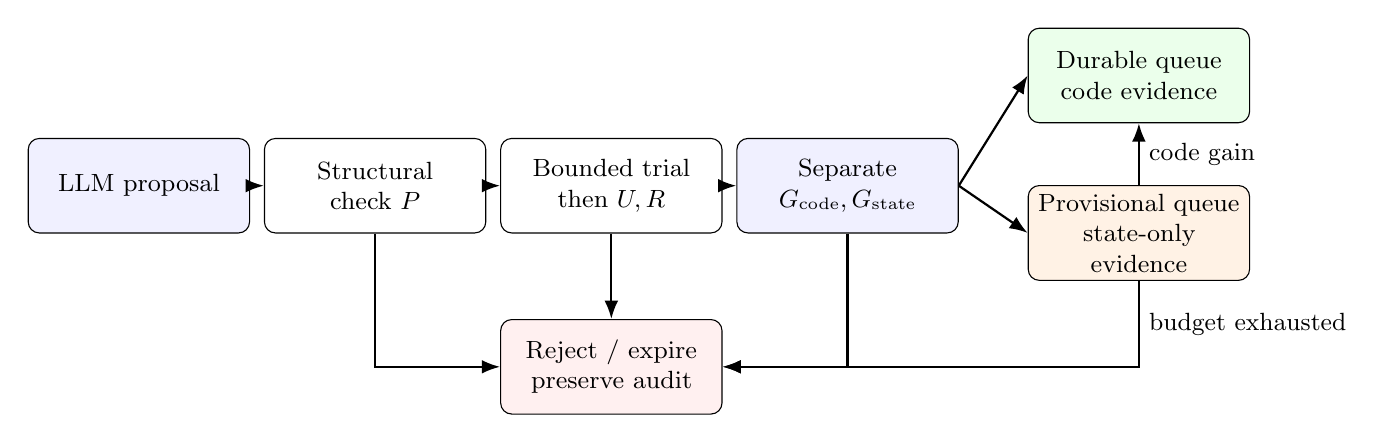
\begin{tikzpicture}[>=Latex,font=\small,
box/.style={draw,rounded corners,align=center,text width=26mm,minimum height=12mm,inner sep=3pt},
arr/.style={->,thick}]
\node[box,fill=blue!6] (llm) at (0,0) {LLM proposal};
\node[box] (p) at (3,0) {Structural\\check $P$};
\node[box] (trial) at (6,0) {Bounded trial\\then $U,R$};
\node[box,fill=blue!6] (gain) at (9,0) {Separate\\$\gcode,\gstate$};
\node[box,fill=green!8] (dur) at (12.7,1.4) {Durable queue\\code evidence};
\node[box,fill=orange!10] (prov) at (12.7,-.6) {Provisional queue\\state-only evidence};
\node[box,fill=red!6] (rej) at (6,-2.3) {Reject / expire\\preserve audit};
\draw[arr] (llm)--(p);
\draw[arr] (p)--(trial);
\draw[arr] (trial)--(gain);
\draw[arr] (gain.east)--(dur.west);
\draw[arr] (gain.east)--(prov.west);
\draw[arr] (p.south)|-(rej.west);
\draw[arr] (trial.south)--(rej.north);
\draw[arr] (gain.south)|-(rej.east);
\draw[arr] (prov.south)|-node[pos=.25,right]{budget exhausted}(rej.east);
\draw[arr] (prov.north)--node[right]{code gain}(dur.south);
\end{tikzpicture}
\caption{Controller contract: $P$ precedes execution; $U/R$ and distinct code/IPSM evidence precede queue disposition. Native saving must not bypass the boundary. Security-oracle artifacts are preserved separately.}
\label{fig:architecture}
\end{figure*}

\subsection{State-selection episodes and independent reward}
An episode begins when the scheduler selects response-derived state $s$ and a seed capable of reaching it. It receives one fixed execution-energy budget. Individual executions within the episode do not generate repeated posterior updates. Mutation counts, reset failures, elapsed time, and budget exhaustion are logged. Infrastructure-interrupted episodes are incomplete, rather than silently assigned reward zero.

For completed episode $t$ targeting $s_t$, let $\Delta B_t$ count previously unseen code branches discovered within that episode. The main reward is
\begin{equation}
r_t=\mathbf{1}\{\Delta B_t>0\}.
\label{eq:reward}
\end{equation}
A declared code-edge instrumentation variant is admissible, but IPSM novelty is excluded. Favored descendants are a secondary sensitivity reward. Equal energy prevents a state appearing more productive merely because it receives more executions. Trial execution, ordinary mutation, and provisional validation use distinct event types to avoid duplicate updates.

$\theta_s$ denotes the probability of positive code reward conditional on selecting $s$ under the episode policy and current campaign phase. It is instrumental utility, not the probability that $s$ is a true semantic state. $U$ continues to mean response acceptability; utility is never denoted $U(s)$.

\subsection{Discounted productivity estimates}
Each state starts with $\alpha_s=\beta_s=1$ and
\begin{equation}
\theta_s\sim\operatorname{Beta}(\alpha_s,\beta_s),\qquad
\widehat{\theta}_{s,t}^{\,\mathrm{pre}}
=\frac{\alpha_{s,t}}{\alpha_{s,t}+\beta_{s,t}}.
\end{equation}
For a completed selected-state episode:
\begin{align}
\alpha_s&\leftarrow1+\gamma(\alpha_s-1)+r_t,\\
\beta_s&\leftarrow1+\gamma(\beta_s-1)+(1-r_t).
\label{eq:update}
\end{align}
The proposed discount is $\gamma=0.995$, with sensitivity values $\{0.99,0.995,1.0\}$. Parameters are frozen after the pilot and before inspecting formal results. At $\gamma=1$, updates reduce to cumulative Beta--Bernoulli counts. For $\gamma<1$, excess prior counts are discounted to respond to changing productivity as coverage saturates.

The term productivity posterior denotes this discounted working model. With discounting it is not the exact posterior of a stationary Bernoulli process. Discounting occurs on completed episodes for the selected state; unselected states do not automatically age in wall-clock time. The update clock and cold start are therefore explicit applicability limits.

Every calibration metric uses the pre-update mean recorded before reward. Post-update predictions would leak the outcome into their own evaluation. Thompson samples are recorded separately and are not substituted for predicted Bernoulli probabilities in reliability calculations.

\subsection{Calibrated scheduling}
The topology term favors underexplored observed states:
\begin{equation}
F(s)=
\begin{cases}
4,&s\text{ is newly reachable or }\deg^+(s)\leq1,\\
2,&1<\deg^+(s)\leq3,\\
1,&\deg^+(s)>3.
\end{cases}
\end{equation}
Only reachable states with eligible seeds participate. $\deg^+(s)$ counts outgoing IPSM state edges, not code branches. Let $B(s)$ denote the inherited base weight shared by C, D, and E. Define
\begin{equation}
\operatorname{Frontier}(s)=B(s)F(s).
\end{equation}
Keeping this factor and any warm-up policy fixed prevents calibration from simultaneously changing the baseline scheduler. Draw
\begin{equation}
\widetilde{\theta}_s\sim\operatorname{Beta}(\alpha_s,\beta_s)
\end{equation}
and calculate
\begin{equation}
S(s)=\operatorname{Frontier}(s)[\epsilon+(1-\epsilon)\widetilde{\theta}_s],
\qquad\epsilon=0.1.
\label{eq:score}
\end{equation}
Select a state with probability proportional to $S(s)$, recording the pseudorandom seed. This is Thompson-sampled weighted selection, not an argmax policy. Under a finite eligible set, the positive floor gives nonzero selection probability, not a fixed number of selections.

The fixed-policy comparator retains the original penalty:
\begin{equation}
S_D(s)=\operatorname{Frontier}(s)\rho_{\mathrm{fixed}}(s).
\end{equation}
Its cached queue-yield ratio $p_s=D_s/(N_s+1)$ counts interesting queued paths $D_s$ per state selections $N_s$. It is not a calibrated Bernoulli probability and can reflect state-only novelty or unequal execution energy. E replaces only $\rho_{\mathrm{fixed}}$ with the calibrated factor in Equation~\ref{eq:score}, preserving the shared base, admission, prompts, triggers, repair settings, and caps. The source implementation's integer score conversion and initial round-robin cycles require explicit freezing and verification before comparison.

\begin{figure}[t]
\centering
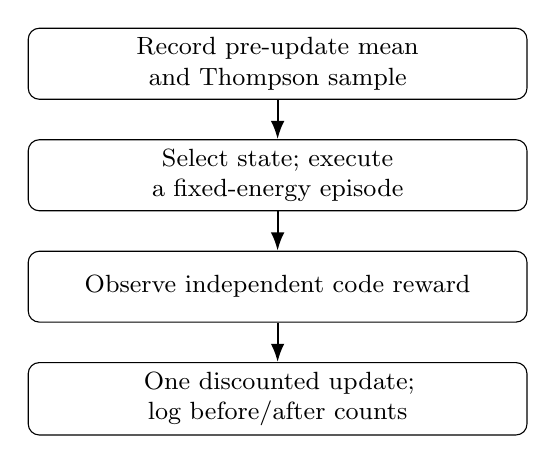
\begin{tikzpicture}[>=Latex,font=\small,
box/.style={draw,rounded corners,align=center,text width=61mm,minimum height=9mm},
arr/.style={->,thick}]
\node[box] (pre) {Record pre-update mean and Thompson sample};
\node[box,below=5mm of pre] (run) {Select state; execute a fixed-energy episode};
\node[box,below=5mm of run] (reward) {Observe independent code reward};
\node[box,below=5mm of reward] (update) {One discounted update; log before/after counts};
\draw[arr](pre)--(run);\draw[arr](run)--(reward);\draw[arr](reward)--(update);
\end{tikzpicture}
\caption{Productivity calibration: prediction precedes reward. IPSM state-edge growth is diagnostic and excluded from the main reward.}
\label{fig:posterior}
\end{figure}

\begin{algorithm}[t]
\small\caption{Evidence-gated candidate processing}\label{alg:admission}
\DontPrintSemicolon
\KwIn{Candidate $x$, target, immutable pre-trial snapshot}
Record candidate, prompt, reply, and lineage identifiers\;
\If{$\neg P(x)$}{Record structural rejection; stop processing $x$\;}
Execute one bounded trial without durable queue insertion\;
Record $U,R,\gcode,\gstate$ and reason codes\;
\If{$P\land U\land R\land\gcode$}{Promote $x$ to $Q_{\mathrm{dur}}$\;}
\ElseIf{$P\land U\land R\land\neg\gcode\land\gstate$}{
Insert $x$ into $Q_{\mathrm{prov}}$\;
\While{budget, validation deadline, and campaign time remain}{
Check budget before the next descendant execution\;
Execute and record one descendant\;
\If{qualifying code gain and validation pass}{
Record first productive descendant; promote; end validation\;
}
}
Record expiration or campaign censoring if still provisional\;
}
\Else{Record rejection\;}
Preserve security-oracle evidence separately\;
\end{algorithm}

\subsection{Intervention policy and optional repair}
Plateau assistance uses a frozen definition, cadence, counters, and retry policy. The legacy trigger combines IPSM state-edge growth with an unproductive streak. If retained, its dependence on the proxy remains common to the causal arms and is reported; calibrating scheduling does not automatically calibrate triggering.

Repair is disabled in primary C/D/E comparisons. Counterexample-guided local repair remains an optional implementation feature evaluated diagnostically. E-with-repair versus E-without-repair records failure type, counterexample, parent repair ID, before/after hypothesis hashes, changed fields, validation, post-repair predicates, descendant gain, and token/latency cost. Sparse events or illustrative examples do not establish an effect. An additional contribution would require sufficient events, reproducible code gains, and independent statistical support across several targets.


\section{Implementation and Evidence Status}
\label{sec:implementation}
The source includes split gain fields, provisional-queue machinery, and a posterior-scheduling switch. Their presence does not establish that archived runs exercised or correctly enforced the intended mechanisms. Run configuration, execution ordering, and event semantics must be checked together.

Several differences are material. The candidate path invokes native execution before evaluating the post-trial gate; native execution can already save a code-novel input. A later $U/R$ failure does not undo that insertion, so the inspected implementation does not strictly enforce Equation~\ref{eq:admission}. Native bitmap novelty includes hit-count changes, rather than exclusively new code branches. Provisional accounting checks budgets after a complete fuzzing round and can overshoot the nominal limits.

In addition, trial IPSM novelty is computed from graph updates tied to queue saving. In the inspected ordinary gated path, an unsaved candidate does not independently update that graph before the state-only check, whereas a native save already supplies code evidence. This ordering obstructs the intended state-only provisional branch. Zero provisional records therefore cannot be interpreted as successful filtering or proof that provisional validation is unnecessary.

Existing $P$ flags can reflect action-schema acceptance rather than complete wire-format validation. The $R$ implementation also admits generic parsed transitions without requiring the intended target/frontier. These are weaker conditions than the design definitions. Table~\ref{tab:implementation} summarizes the boundaries. This manuscript revision does not change fuzzer code; it separates the proposed contract from the implementation evidence.

\begin{table*}[t]
\centering\small
\caption{Controller contract versus inspected implementation and available evidence. Source findings describe the current checkout; archive/source identity is not assumed without a commit or binary hash.}
\label{tab:implementation}
\begin{tabularx}{\textwidth}{Y Y Y}
\toprule
Contract & Current boundary & Evaluation consequence \\
\midrule
Gate precedes durable promotion & Native saving may precede post-trial $U/R$ checks. & Disposition/reason text does not certify strict queue protection. \\
Independent state-only trial evidence & IPSM update depends on saving in the inspected path. & Zero provisional events cannot establish a low state-only rate. \\
Full structural and reachability checks & $P$ can mean action schema; $R$ accepts generic state transitions. & Audit exact parser and target-hit evidence. \\
Main reward is new code coverage & Bitmap novelty includes hit-count changes; some named branch fields count bitmap slots. & Keep offline branches, bitmap slots, and save events distinct. \\
Fixed-energy episode & Existing rounds vary mutation energy and may include zero-execution attempts. & Raw episode productivity is not equal-opportunity productivity. \\
Strict provisional budget & Limits checked after a whole fuzzing round. & Nominal 64/30-second thresholds are not enforced maxima. \\
Verified run configuration & Start event is written before some environment flags are parsed. & Cross-check launcher, end records, and effective execution path. \\
Equal total call/token caps & The logged 64 cap concerns plateau use; token-cap logging does not prove enforcement. & No existing total-budget fairness claim. \\
Repair disabled in C/D/E & Code defaults and activation differ from the prospective configuration. & Legacy labels do not certify the complete D-arm contract. \\
\bottomrule
\end{tabularx}
\end{table*}

\subsection{Append-only event contract}
Six core streams record run configuration, candidate generation, admission trials, provisional lifecycle, state-selection episodes, and bug-oracle events. Repair adds a seventh optional stream. Table~\ref{tab:events} specifies joinable fields. Missing fields are not replaced with zero.

\begin{table*}[t]
\centering\footnotesize
\caption{Required logging schema. Each event also includes run ID, schema version, event sequence, and timestamp. Required fields are not claimed to be fully present in the current archive.}
\label{tab:events}
\begin{tabularx}{\textwidth}{l Y}
\toprule
Stream & Minimum additional fields \\
\midrule
\texttt{run\_config} & Arm; target/fuzzer commits; image digest; model/version/endpoint; temperature, top-$p$, penalties; call/token caps; seed; CPU/memory quota; start/end; termination reason. \\
\texttt{candidate\_event} & Candidate/prompt IDs; prompt/raw-reply hashes; raw candidate or artifact path; action; input/output tokens; source/requested states; generation timestamp; parent candidate. \\
\texttt{admission\_trial} & Candidate/trial IDs; $P/U/R$ and reasons; response code/hash; timeout/reset/drop; state sequence; target/frontier reached; pre/post IPSM nodes/state edges and code coverage; favored reason; latency; disposition. \\
\texttt{provisional\_event} & Stable candidate/provisional IDs; budget; actual descendant executions/code gain; first productive descendant; conversion timestamp; promotion latency; expiration/censoring reason. \\
\texttt{state\_selection\_episode} & Episode/state/seed IDs; pre-update $\alpha,\beta,\widehat{\theta}$; Thompson sample; frontier/final score; mutations; code-branch/IPSM state-edge gain; reward; post-update $\alpha,\beta$; latency; completion status. \\
\texttt{bug\_event} & Anonymous oracle ID; reached/triggered; first trigger time; reproducing input; vulnerable/patched result; sanitizer evidence; root-cause signature. CVE identity remains isolated metadata. \\
\texttt{repair\_event} (optional) & Repair/parent IDs; failure/counterexample; before/after hypothesis hashes; changed field; validation before/after; post-repair predicates/descendant gain; tokens/latency. \\
\bottomrule
\end{tabularx}
\end{table*}

Before formal runs, candidate-event completeness must reach at least 99.9\%; no trial may lack a candidate ID, no posterior update may lack an episode ID, and every promotion must be reconstructable. Completeness denominators include failed generation and parsing paths, not only successful candidates. File presence, join completeness, and agreement between logged disposition and actual queue state are separate checks.

\section{Experimental Protocol}
\label{sec:protocol}
This protocol is prospective for unfinished confirmatory experiments. The supplied archive does not establish a dated preregistration, parameter freeze, or completed pilot. We do not retrospectively call it preregistered. A version, timestamp, and checksum must be frozen before the remaining runs, with subsequent deviations recorded. Development and pilot observations remain separate.

\subsection{Research questions}
\begin{enumerate}
\item \textbf{RQ1: State/code alignment.} How reliably does response-derived state novelty predict downstream code progress across targets and campaign phases? Measure IPSM state-edge/code-branch alignment, episode productivity, calibration, and boundary cases.
\item \textbf{RQ2: Admission.} Does execute-before-promote reduce durable queue pollution and improve downstream productivity under matched proposal and scheduling conditions? Compare D with C.
\item \textbf{RQ3: Calibration.} Does online productivity calibration improve scheduling over a fixed response-state heuristic? Compare E with D.
\item \textbf{RQ4: Historical vulnerability rediscovery.} Does the controller improve reproducible rediscovery under independent reached/triggered oracles and patch validation?
\item \textbf{RQ5: Cost and applicability.} What runtime, throughput, and LLM costs arise, and under which target characteristics does the method fail to help?
\end{enumerate}
The directional hypotheses are improved downstream productivity for D over C and improved code-branch AUC for E over D. Regressions, null results, and uncertainty are reported per target rather than hidden in pooled means or replaced by increased IPSM state-edge counts.

\subsection{Five arms and causal comparisons}
\begin{table*}[t]
\centering\small
\caption{Confirmatory arm matrix. Repair is disabled in C/D/E. Names specify required configurations, not inferred identities from archive filenames.}
\label{tab:arms}
\begin{tabularx}{\textwidth}{l c Y Y Y}
\toprule
Arm & LLM & Admission & Scheduler & Role \\
\midrule
A: AFLNet & No & Native AFLNet & AFLNet & Non-LLM baseline. \\
B: Controlled ChatAFL & Yes & ChatAFL direct/open-loop & ChatAFL lineage & B--A: total controlled LLM-lineage change. \\
C: LoopFuzz-direct & Yes & Parseable candidates directly durable & Fixed LoopFuzz & Admission counterfactual. \\
D: LoopFuzz-gated-fixed & Yes & Evidence gate + provisional queue & Same fixed LoopFuzz & D--C: admission effect. \\
E: LoopFuzz-gated-calibrated & Yes & Identical to D & Productivity calibration & E--D: scheduling calibration. \\
\bottomrule
\end{tabularx}
\end{table*}

C/D share model configuration, prompt construction, trigger, repair setting, scheduler, and budget policy; the intended intervention is admission. E/D share admission and differ only in state selection. Controlled ChatAFL retains its scheduling lineage; replacing it with the LoopFuzz scheduler would change the baseline. B--A is not an isolated admission comparison.

Proposal control has two scopes. A paired candidate diagnostic evaluates the same recorded output from the same target/campaign snapshot under direct and gated admission with identical descendant budgets. It supports a candidate-level counterfactual. Independent online campaigns diverge in queue and state history, so matching policies cannot guarantee identical prompt bytes or model outputs throughout. Recorded-action replay supports parser checks, predicate replay, snapshot comparisons, and provider-free artifact inspection; it does not make a replayed campaign equivalent to live adaptation.

\subsection{Targets, builds, and resource controls}
The primary design contains nine servers: four FTP servers, Exim (SMTP), Live555 (RTSP), Kamailio (SIP), Forked-daapd (DAAP/DACP over HTTP), and Lighttpd1 (HTTP). Exact build metadata unavailable for a verified comparison remains blank in Table~\ref{tab:targets}. Hardware settings and version pins are not carried over from the old manuscript without evidence linking them to the present runs.

\begin{table*}[t]
\centering\small
\caption{Target/protocol/build matrix. Blank build fields await exact commit, image, coverage, and reset manifests.}
\label{tab:targets}
\begin{tabularx}{\textwidth}{l l Y Y Y}
\toprule
Target & Protocol & Commit/version & Image digest & Coverage build / reset hook \\
\midrule
LightFTP & FTP & \missing & \missing & \missing \\
bftpd & FTP & \missing & \missing & \missing \\
ProFTPD & FTP & \missing & \missing & \missing \\
Pure-FTPd & FTP & \missing & \missing & \missing \\
Exim & SMTP & \missing & \missing & \missing \\
Live555 & RTSP & \missing & \missing & \missing \\
Kamailio & SIP & \missing & \missing & \missing \\
Forked-daapd & DAAP/DACP & \missing & \missing & \missing \\
Lighttpd1 & HTTP & \missing & \missing & \missing \\
\bottomrule
\end{tabularx}
\end{table*}

Each causal comparison uses the same source revision, flags, instrumentation, seeds, replay procedure, and reset policy. Launch order is randomized within host blocks and balanced across machines and periods. Runs record fuzzer seeds, quotas, measured CPU use, throttling, and execution rates. Container quotas alone do not establish equal CPU time. Startup, model waiting, admission trials, provisional descendants, and cleanup enter the resource ledger.

Each arm initially receives 10 independent 24-hour runs per target; C/D/E receive 10 more, reaching 20 each. For nine targets and one allocated CPU per run, the stages require 10,800 and 6,480 CPU-hours, totaling 17,280 before overhead/failures. These are planned resources, not measured usage. A four-target pilot covers Forked-daapd, Lighttpd1, LightFTP, and ProFTPD or Pure-FTPd with five arms, three runs, and four to six hours each. Pilot observations are excluded from formal inference.

The intention-to-run ledger includes planned, launched, completed, timeout, target/fuzzer crash, infrastructure failure, extraction failure, excluded, and rerun states, with reasons and linked attempts. Poor coverage is never an exclusion criterion. Only predefined infrastructure failures permit reruns, and original launches remain visible. An interrupted run is not silently extended to 24 hours. It contributes a declared failure outcome or censored observation according to the estimand, with sensitivity analysis; completed-run-only results are not intention-to-run results.

\subsection{LLM fairness and configuration}
The main design uses equal policy and equal ceilings. All LLM arms must use identical model configurations, intervention policies, and resource ceilings. Actual calls and token usage are reported because adaptive trajectories can trigger different numbers of interventions. Table~\ref{tab:llm} does not invent unfrozen settings.

\begin{table*}[t]
\centering\small
\caption{Shared LLM configuration required for B--E. Blank values await the confirmatory freeze; historical settings do not fill these cells.}
\label{tab:llm}
\begin{tabularx}{\textwidth}{Y c Y}
\toprule
Field & Frozen value & Required handling \\
\midrule
Provider / endpoint / immutable model version & \missing & Record resolved version; an alias alone is insufficient. \\
Temperature by call class & \missing & Match corresponding call classes across arms. \\
Top-$p$ / presence and frequency penalties & \missing & Explicit values or documented provider defaults. \\
Maximum output tokens per attempt & \missing & Shared cap; record truncation and failures. \\
Maximum attempted calls / total tokens & \missing & Include all classes and retries. \\
Timeout / retry count / backoff & \missing & Fixed policy; record realized waits and failures. \\
Model-side seed / support status & \missing & Record support; do not promise service determinism. \\
Prompt corpus / template version & \missing & Shared information policy; prompt/reply hashes. \\
Plateau cadence / threshold / reset & \missing & Same trigger, including state-growth dependencies. \\
\bottomrule
\end{tabularx}
\end{table*}

An output-token cap per request is not a total campaign ceiling. A zero legacy token-cap field must be interpreted through its actual enforcement, not reported as equal-token control. Dollar costs require auditable usage and applicable prices; unknown charges remain blank.

Secondary comparisons report code-branch gain per 1,000 total tokens, per LLM call, at a common cumulative token budget, and at a common call count. Security costs use CPU-hours and 100,000-token units. Accounting includes unsuccessful generations, retries, validation, and optional repair. A fixed intervention schedule provides a cost-control sensitivity, not a replacement for the adaptive main policy. Ratios with zero denominators are undefined.

\subsection{Mechanism and calibration metrics}
For every target/arm, report candidate generation, $P/U/R$ first-failure distribution, direct durable and provisional rates, conversion, expiration, promotion latency, queue size, trial latency, descendant executions, code gain per candidate/token, episode productivity, and throughput. Denominators and incomplete/censored events accompany rates.

Downstream productivity uses a fixed descendant horizon rather than admission gain. For a declared cohort $\mathcal{C}$ of $N$ candidates enrolled before their outcomes are known, let $Y_i(H)=1$ if a later descendant produces new code coverage within $H$ executions, and $0$ if the full horizon is observed without gain. With complete observation, define
\begin{equation}
\operatorname{Productivity@}H=\frac{1}{N}\sum_{i\in\mathcal{C}}Y_i(H).
\end{equation}
Initially $H=64$. The admission trial is excluded. A positive outcome can be established early; a negative requires the complete horizon. With $n_+$ known positives and $n_?$ censored unresolved candidates, report the cohort bounds $[n_+/N,(n_++n_?)/N]$ rather than deleting incomplete negatives from the denominator. The primary paired diagnostic reserves the same full validation horizon for both controllers; incomplete online cohorts are reported with these bounds and censoring counts. Durable and provisional cohorts are distinct; post-promotion productivity uses a fresh horizon. Thus neither admission gain nor selective observation mechanically raises measured productivity.

Avoided queue pollution requires C--D evidence. In the paired diagnostic, identify direct-arm durable candidates without downstream gain and compare their retention under gating. D-arm rejections are not automatically pollution. A random, predeclared sample of rejected candidates receives shadow validation to estimate false negatives, with inclusion probabilities, snapshots, lineage, and cost recorded.

For complete episodes, $p_t=\widehat{\theta}_{s_t,t}^{\,\mathrm{pre}}$ predicts later reward $r_t$. The Brier score is
\begin{equation}
\mathrm{BS}=\frac{1}{n}\sum_{t=1}^{n}(p_t-r_t)^2.
\end{equation}
Expected calibration error (ECE) uses ten fixed equal-width probability bins and reports counts, mean predictions, and observed frequencies. Empty bins stay empty. Reliability plots and AUPRC accompany the score; with no positive episodes AUPRC is undefined. Compare Brier score to a prequential base-rate predictor because rare rewards can make uninformative near-zero predictions look accurate. IPSM state-edge/code-gain ratios with zero code gain are undefined or shown as separate zero-gain cases.

Episodes within a run are dependent; uncertainty is clustered by run and reported by target/phase. Posterior trajectories and state weights are diagnostic, not evidence that every state is accurately learned. Correlation between IPSM growth and later code gain is evaluated within target and phase, without pooling raw counts across unlike programs.

\subsection{Coverage and statistical analysis}
Primary coverage outcomes are code-branch AUC over 24 hours and final code-branch count. AUC uses each run's cumulative time series with a common interpolation convention and instrumentation, in branch-hours. Native endpoints at unequal durations are not substituted. Time to 95\% of a target-specific common reference endpoint uses a threshold frozen before formal comparisons; unreached thresholds are censored.

Per target, report mean, median, dispersion, bootstrap 95\% intervals, two-sided Mann--Whitney U tests, and Cliff's $\delta$. The primary coverage family has 36 tests: nine targets, D--C and E--D, final branches and AUC. Benjamini--Hochberg controls this family at $q=0.05$. The primary admission-mechanism family has nine D--C productivity contrasts and is reported separately. Other diagnostics and sensitivity tests are exploratory. Effect direction is treatment minus comparator.

Cross-target summaries use equal-weight target effects and a hierarchical bootstrap resampling targets, then runs within targets. Raw branch counts from different programs or individual executions are not pooled as independent samples. Target regressions and uncertainty accompany aggregates. Historical time-to-trigger uses Kaplan--Meier estimates, right censoring, and CVE-specific deadline recall. Fuzzer-failure interruptions are distinguished because censoring may be informative.


\section{Available Evidence and Results}
\label{sec:results}
The empirical source for this revision is the supplied \texttt{Key\_Experiment} directory. Earlier selected-run tables, significance counts, auxiliary comparisons, crash-class totals, and curves are not treated as measurements of the new controller. A blank numeric cell below means unavailable or unvalidated evidence, never a measured zero.

\subsection{Archive inventory and observation horizon}
There are 91 AFLNet and 90 LoopFuzz archives. The 18 result manifests enumerate 180 runs, leaving one additional Pure-FTPd AFLNet archive without a matching manifest/status record. One other Pure-FTPd AFLNet run has exit code 1 despite a completed summary label. A result manifest is not a complete record of all planned but unlaunched attempts.

LoopFuzz summaries label 60 runs completed, 12 as SIGABRT, and 18 as exit-code-137 outcomes. The latter label does not independently establish out-of-memory termination or a vulnerability. Runtime in the archived fuzzer statistics spans 410--1522 minutes for LoopFuzz; AFLNet summaries report 1499 minutes. It is fuzzer runtime, not total CPU time or necessarily the full startup-to-cleanup campaign duration.

Run configurations declare fixed-policy LoopFuzz and \texttt{calibration=false}; no separate B, C, or E archive family is supplied. The startup logging-order issue in Table~\ref{tab:implementation} means these declarations require launcher/end-record corroboration. They do not certify complete D-arm conformance. No calibrated-arm effect is inferred from posterior fields alone.

% Generated by audit_experiments.py. All native endpoint rows are retained.
\begin{table*}[t]
\centering\small
\caption{Supplied archive inventory. Completed, SIGABRT, and exit-137 columns refer only to recorded LoopFuzz runs and reproduce the summary labels; exit code 137 is not independent evidence of an out-of-memory failure. Durations are observed fuzzer runtime, in minutes.}
\label{tab:observed_inventory}
\begin{tabular}{lrrrrrl}
\toprule
Target & AFLNet & LoopFuzz & Completed & SIGABRT & Exit 137 & LoopFuzz duration \\
\midrule
LightFTP & 10 & 10 & 10 & 0 & 0 & 1507--1522 \\
bftpd & 10 & 10 & 3 & 0 & 7 & 1499--1510 \\
ProFTPD & 10 & 10 & 3 & 0 & 7 & 1489--1512 \\
Pure-FTPd & 11 & 10 & 6 & 0 & 4 & 1460--1472 \\
Exim & 10 & 10 & 10 & 0 & 0 & 1477--1486 \\
Live555 & 10 & 10 & 10 & 0 & 0 & 1501--1505 \\
Kamailio & 10 & 10 & 7 & 3 & 0 & 1055--1481 \\
Forked-daapd & 10 & 10 & 2 & 8 & 0 & 410--1499 \\
Lighttpd1 & 10 & 10 & 9 & 1 & 0 & 985--1485 \\
\bottomrule
\end{tabular}
\end{table*}
\begin{table*}[t]
\centering\small
\caption{Exploratory native terminal endpoints (mean $\pm$ sample standard deviation), retaining every supplied summary row, including early terminations. These values are not matched-deadline or causal A--E comparisons.}
\label{tab:observed_endpoints}
\begin{tabular}{lrrrr}
\toprule
& \multicolumn{2}{c}{Code branches (\texttt{b\_abs})} & \multicolumn{2}{c}{IPSM state edges} \\
Target & AFLNet & Recorded LoopFuzz & AFLNet & Recorded LoopFuzz \\
\midrule
LightFTP & $71.9 \pm 2.8$ & $71.1 \pm 0.3$ & $185.6 \pm 12.4$ & $212.1 \pm 12.4$ \\
bftpd & $486.0 \pm 8.8$ & $502.7 \pm 7.5$ & $163.1 \pm 15.4$ & $226.7 \pm 14.0$ \\
ProFTPD & $5053.8 \pm 97.4$ & $5404.6 \pm 95.6$ & $190.5 \pm 27.9$ & $307.4 \pm 18.6$ \\
Pure-FTPd & $1076.4 \pm 89.6$ & $1223.3 \pm 29.7$ & $236.5 \pm 26.7$ & $321.4 \pm 11.1$ \\
Exim & $3798.8 \pm 43.3$ & $3914.9 \pm 20.9$ & $88.8 \pm 5.2$ & $152.7 \pm 9.3$ \\
Live555 & $2893.6 \pm 14.5$ & $3057.9 \pm 22.0$ & $96.1 \pm 8.6$ & $171.9 \pm 11.3$ \\
Kamailio & $10002.6 \pm 144.2$ & $10660.3 \pm 230.5$ & $109.4 \pm 9.7$ & $134.3 \pm 15.4$ \\
Forked-daapd & $2330.8 \pm 60.0$ & $2662.6 \pm 151.4$ & $21.6 \pm 2.1$ & $21.8 \pm 2.3$ \\
Lighttpd1 & $1940.7 \pm 21.2$ & $2126.0 \pm 15.0$ & $17.7 \pm 2.5$ & $29.7 \pm 1.3$ \\
\bottomrule
\end{tabular}
\end{table*}
\begin{table*}[t]
\centering\small
\caption{Observed schema-v2 logging counts from all 90 supplied LoopFuzz archives. Reject, provisional, and durable are recorded decision labels, not verified post-execution queue membership.}
\label{tab:observed_log_counts}
\begin{tabular}{lrrrrrr}
\toprule
Target & Candidates & Trials & Reject & Provisional & Durable & Episodes \\
\midrule
LightFTP & 29 & 29 & 27 & 0 & 2 & 9587 \\
bftpd & 13 & 13 & 13 & 0 & 0 & 3249 \\
ProFTPD & 0 & 0 & 0 & 0 & 0 & 1911 \\
Pure-FTPd & 173 & 173 & 166 & 0 & 7 & 5378 \\
Exim & 24 & 24 & 24 & 0 & 0 & 2650 \\
Live555 & 778 & 778 & 771 & 0 & 7 & 7128 \\
Kamailio & 58 & 55 & 54 & 0 & 1 & 5469 \\
Forked-daapd & 143 & 135 & 135 & 0 & 0 & 4715 \\
Lighttpd1 & 392 & 392 & 392 & 0 & 0 & 19496 \\
\bottomrule
\end{tabular}
\end{table*}


Table~\ref{tab:observed_endpoints} retains every summary row, including interruptions. Its native terminal \texttt{b\_abs} comes from the final available coverage-replay observation; its IPSM state-edge count comes from the final plotting record. These observations are descriptive, not matched 24-hour outcomes. Sample standard deviations express variation among the supplied rows; neither causal claims nor significance tests are attached to unequal-duration endpoints.

\subsection{RQ1: Current alignment observations}
Forked-daapd has mean native code-branch endpoints of $2330.8\pm60.0$ for AFLNet and $2662.6\pm151.4$ for recorded LoopFuzz, while IPSM state-edge endpoints are $21.6\pm2.1$ and $21.8\pm2.3$. This direction does not reproduce the older motivating claim of code regression. The difference cannot be attributed to calibration, which is not established as active.

Lighttpd1 increases in both native metrics: code branches from $1940.7\pm21.2$ to $2126.0\pm15.0$, and IPSM state edges from $17.7\pm2.5$ to $29.7\pm1.3$. These aggregate observations do not demonstrate the hypothesized small state expansion with hidden code progress. LightFTP has near-equal code endpoints, $71.9\pm2.8$ versus $71.1\pm0.3$, with larger recorded LoopFuzz IPSM state-edge counts, $185.6\pm12.4$ versus $212.1\pm12.4$. That pattern motivates a saturation analysis but does not establish the full time course or identify individual misleading states.

All three cases require common-build, common-horizon verification and event joins before becoming mechanism evidence. State-level posterior evolution, predicted-versus-observed productivity, and weights of code-unproductive states require validated calibrated episodes. \figref{fig:reliability} therefore remains blank.

\begin{figure}[t]
\centering\blankpanel{28mm}
\caption{Reserved reliability diagram: pre-update predicted episode productivity versus observed code reward, with bin counts, run-clustered uncertainty, Brier score, ECE, and AUPRC. No conforming calibrated-arm observations are available.}
\label{fig:reliability}
\end{figure}

\subsection{RQ2: Observed admission records and missing counterfactual}
The archive contains 1,610 candidate records, 1,599 trial records, 1,582 reject labels, 17 durable labels, and no provisional labels. Eleven candidate records lack a trial match: eight for Forked-daapd and three for Kamailio. The observed join rate is 99.32\%; this is neither the required 99.9\% event-completeness demonstration nor a measure of unlogged generation opportunities. No trial lacks a matching candidate among the parsed records.

Candidate/admission files occur in 69 of 90 LoopFuzz archives; ProFTPD has none despite nonzero model-call counters. All 90 archives lack provisional and repair lifecycle files. Table~\ref{tab:observed_log_counts} reports observed record counts. Zero recorded lifecycle events do not yield a zero conversion rate or prove absence of repair/provisional behavior.

Disposition labels are not independently verified queue membership. The native-save ordering and state-only reachability problems prevent interpreting rejected labels as avoided queue pollution or durable labels as proof of strict predicate conformance. Without C--D and descendant lineage, downstream productivity, shadow-validation false negatives, and avoided nonproductive retention remain blank.

\subsection{RQ3: Scheduling evidence and unfilled causal results}
The 90 LoopFuzz archives contain 59,583 episode records. Their recorded execution counts range from zero to 17,080, which is not a shared fixed-energy measurement surface. Some coverage fields are named as code branches or code edges while the inspected implementation fills bitmap-slot counts or coverage-save-event counts. These values cannot be merged with source-level \texttt{b\_abs} or treated as the main reward of Equation~\ref{eq:reward}.

A fixed scheduler can log and update productivity estimates without using Thompson selection. The presence of a \texttt{sampled\_theta} field therefore does not establish E-arm execution. No D--E experiment supports a calibration benefit. Table~\ref{tab:mainresults} leaves all unvalidated confirmatory cells blank, including baseline cells not yet certified at the common horizon and build.

\begin{table*}[t]
\centering\small
\caption{Confirmatory final code-branch count / code-branch AUC (branch-hours). Planned runs per target: A/B, 10; C/D/E, 20. Cells await comparable experiments and run-level inference.}
\label{tab:mainresults}
\begin{tabularx}{\textwidth}{l *{5}{>{\centering\arraybackslash}X}}
\toprule
Target & A & B & C & D & E \\
\midrule
LightFTP & \missing & \missing & \missing & \missing & \missing \\
bftpd & \missing & \missing & \missing & \missing & \missing \\
ProFTPD & \missing & \missing & \missing & \missing & \missing \\
Pure-FTPd & \missing & \missing & \missing & \missing & \missing \\
Exim & \missing & \missing & \missing & \missing & \missing \\
Live555 & \missing & \missing & \missing & \missing & \missing \\
Kamailio & \missing & \missing & \missing & \missing & \missing \\
Forked-daapd & \missing & \missing & \missing & \missing & \missing \\
Lighttpd1 & \missing & \missing & \missing & \missing & \missing \\
\bottomrule
\end{tabularx}
\end{table*}

\begin{figure*}[t]
\centering\blankpanel{35mm}
\caption{Reserved code-branch trajectories for A--E under shared instrumentation and a 24-hour horizon. Each target will have its own labeled scale, run-level uncertainty, and incomplete-run accounting. Earlier curves are not reused for the new arms.}
\label{fig:trajectories}
\end{figure*}

\begin{table*}[t]
\centering\small
\caption{Confirmatory mechanism metrics, reported per target. Numeric cells await joined candidate/descendant evidence.}
\label{tab:mechanisms}
\begin{tabularx}{\textwidth}{Y c c c Y}
\toprule
Metric & C & D & E & Denominator / interpretation \\
\midrule
Candidates; $P/U/R$ failure distribution & \missing & \missing & \missing & Distinct IDs; first-failure and joint flags. \\
Direct durable rate & \missing & \missing & \missing & All generated request candidates. \\
State-only provisional rate & \missing & \missing & \missing & All candidates; not enabled for C. \\
Provisional conversion / expiration & \missing & \missing & \missing & Provisional admissions, including pending/censored counts. \\
Promotion / trial latency & \missing & \missing & \missing & Measured time, including failed trials. \\
Downstream productivity@64 & \missing & \missing & \missing & Later descendants, excluding admission gain. \\
Queue size / nonproductive retention & \missing & \missing & \missing & Queue state plus C--D counterfactual. \\
Shadow-validation false-negative rate & \missing & \missing & \missing & Random rejected-candidate sample. \\
Code-branch gain per episode & \missing & \missing & \missing & Completed equal-energy episodes. \\
Brier / ECE / AUPRC & \missing & \missing & \missing & Pre-update probabilities; no fabricated fixed-arm probability. \\
Code gain per candidate / 1,000 tokens & \missing & \missing & \missing & Joined gain and complete usage. \\
\bottomrule
\end{tabularx}
\end{table*}

\begin{figure}[t]
\centering\blankpanel{26mm}
\caption{Reserved candidate disposition plot: $P/U/R$ failures, provisional/direct durable admission, conversion, expiration, and censoring. Counts must reconcile with the candidate ledger and actual queue state.}
\label{fig:dispositions}
\end{figure}

\subsection{RQ5: Recorded costs and interpretation limits}
The final saved statistics across 90 LoopFuzz runs report 13,563 model calls, 10,237,947 prompt tokens, and 9,233,121 completion tokens, totaling 19,471,068 tokens. Calls range from 37 to 248 per run. Thus the logged cap of 64 is not an enforced all-call campaign ceiling. These are saved tool counters, not independently reconciled provider billing. Some final aggregate statistics lag the event stream, so costs may omit the last reporting window.

Recorded configurations include a model alias, grammar/plateau temperatures of 0.5/1.2, top-$p$ 1.0, maximum output tokens 4096, and total-token-cap field 0. The alias does not establish an immutable provider model. Startup configuration timing and missing build/resource provenance limit interpretation. These historical values do not fill the prospective shared configuration in Table~\ref{tab:llm}.

Candidate token fields do not necessarily cover all call classes or retries; summing them is not total campaign cost. Low-activation targets, high-rejection targets, token outliers, saturation, and regressions must remain in the final analysis. Low activation may reflect productive mutation or a restrictive trigger; high rejection may reflect either useful gating or false negatives. Both need mechanism evidence.

% Generated from the final saved fuzzer_stats snapshots, not provider billing.
\begin{table}[t]
\centering\small
\caption{Recorded LoopFuzz costs: per-run minimum--maximum across all ten supplied runs per target. Total tokens combine prompt and completion tokens; k denotes 1,000 tokens. Final saved snapshots may omit the last reporting window and are not reconciled provider billing.}
\label{tab:observed_costs}
\begin{tabular}{lrr}
\toprule
Target & Model calls & Total tokens (k) \\
\midrule
LightFTP & 156--161 & 174.9--224.7 \\
bftpd & 199--248 & 198.0--301.8 \\
ProFTPD & 188--192 & 170.1--198.8 \\
Pure-FTPd & 207--242 & 200.2--264.1 \\
Exim & 106--123 & 109.4--151.0 \\
Live555 & 123--151 & 264.1--329.7 \\
Kamailio & 56--65 & 157.0--183.2 \\
Forked-daapd & 37--163 & 124.1--540.9 \\
Lighttpd1 & 131--181 & 168.5--241.4 \\
\bottomrule
\end{tabular}
\end{table}


\begin{figure}[t]
\centering\blankpanel{28mm}
\caption{Reserved cost-performance comparison: code coverage and CVE recall versus total tokens and measured CPU-hours, with uncertainty. No efficiency frontier is inferred from incomplete usage or unmatched arms.}
\label{fig:cost}
\end{figure}

\begin{table}[t]
\centering\small
\caption{Optional repair diagnostics. Repair is outside primary causal comparisons; unavailable observations stay blank.}
\label{tab:repair}
\begin{tabularx}{\columnwidth}{Y c c}
\toprule
Metric & E, repair off & E, repair on \\
\midrule
Repair opportunities / attempts & \missing & \missing \\
Before/after validation success & \missing & \missing \\
Post-repair descendant code gain & \missing & \missing \\
Changed fields / locality & \missing & \missing \\
Token / latency cost & \missing & \missing \\
Independent effect / interval & \missing & \missing \\
\bottomrule
\end{tabularx}
\end{table}

\section{Historical Vulnerability Rediscovery}
\label{sec:cve}
Security outcomes use information-controlled rediscovery of historical vulnerabilities. Previously unknown vulnerabilities are not an optimization objective. Crash seeds, stack hashes, sanitizer messages, and protocol anomalies support triage; they are not independently counted vulnerabilities.

\subsection{Vulnerable/patch-paired benchmark}
For each vulnerability, construct a vulnerable base commit and the same base plus the minimal upstream security patch. Dependencies, flags, instrumentation, configuration, and input compatibility remain identical. Arbitrary old/new releases would confound the patch with unrelated changes.

Eligibility requires a documented historical vulnerability, an identifiable upstream patch, a network-protocol trigger, stable container builds, an independent oracle, compatible vulnerable/patched inputs, and no complex manual setup or exploit seed. Local-file-only or command-line-only bugs do not qualify.

The initial pilot contains six pairs across at least three protocols. Each pair must reach at least 95\% oracle reproducibility in a declared number of validation attempts, show no corresponding patched-target activation, and support automatic build/reset/cleanup without information leakage. Expansion toward twelve follows only after these conditions hold. These are planned sizes, not completed CVEs; Table~\ref{tab:cve} contains no invented identifiers.

\begin{table*}[t]
\centering\small
\caption{Historical vulnerability benchmark template. Six initial slots are reserved; identity, revision, oracle, and validation fields await evidence. Expansion toward twelve is conditional on pilot stability.}
\label{tab:cve}
\begin{tabularx}{\textwidth}{c Y Y Y Y c c}
\toprule
Slot & CVE / protocol & Vulnerable base & Security patch & Oracle / root cause & Repeatability & Patched activation \\
\midrule
1 & \missing & \missing & \missing & \missing & \missing & \missing \\
2 & \missing & \missing & \missing & \missing & \missing & \missing \\
3 & \missing & \missing & \missing & \missing & \missing & \missing \\
4 & \missing & \missing & \missing & \missing & \missing & \missing \\
5 & \missing & \missing & \missing & \missing & \missing & \missing \\
6 & \missing & \missing & \missing & \missing & \missing & \missing \\
\bottomrule
\end{tabularx}
\end{table*}

\subsection{Information control and ground-truth oracles}
CVE identifiers and security advisories are excluded from prompts and RFC corpora. Seeds contain no proof-of-concept exploit. The fuzzer cannot read patches, and benchmark metadata remains isolated. Where possible, a separate preparer assigns anonymous oracle IDs. This is information-controlled rediscovery, not fully blinded discovery: the preparer knows the vulnerability and model pretraining may include public information.

Reaching means visiting vulnerability-related code; triggering means the defined bug condition actually holds. Oracle priority is a source-level trigger predicate, sanitizer evidence, deterministic crash with patch validation, protocol semantic invariant, or reproducible vulnerable/patched behavioral difference. Covering a patched line is insufficient. Root-cause IDs deduplicate repeated triggers and crash manifestations.

Targets bind to localhost or isolated container networks, have no external network access, run without privileged containers, and use disposable state. Every trial resets the target. Release excludes unsanitized exploit corpora. These are benchmark requirements, not inferred properties of the supplied runs.

\subsection{RQ4 outcomes and censoring}
For each CVE and arm, report deadline rediscovery probability, time-to-trigger, reached-but-not-triggered outcomes, patched-target activation, and unique oracle/root-cause IDs. Record code coverage, executions, and tokens before the first trigger, and report CVEs per CPU-hour and 100,000 tokens. The formal rediscovery plan uses ten runs per arm with a declared 12-hour deadline frozen before execution.

Runs without triggers are right-censored at the observed deadline; interruptions are distinguished from ordinary deadline censoring. Kaplan--Meier curves are CVE-specific or explicitly stratified. Unlike vulnerabilities are not naively pooled as identical events. No normalized vulnerable/patch-paired result is established by the current archive, so \figref{fig:km} and Table~\ref{tab:cveresults} remain blank.

\begin{figure}[t]
\centering\blankpanel{28mm}
\caption{Reserved Kaplan--Meier time-to-trigger curves with risk sets, censoring marks, and a common deadline. Crash-file counts are not converted into rediscovery events.}
\label{fig:km}
\end{figure}

\begin{table*}[t]
\centering\small
\caption{Historical rediscovery outcomes, to be reported by CVE and arm. Blank cells indicate missing validated vulnerable/patch-paired evidence.}
\label{tab:cveresults}
\begin{tabularx}{\textwidth}{Y *{5}{>{\centering\arraybackslash}X}}
\toprule
Outcome & A & B & C & D & E \\
\midrule
CVE-level recall by deadline & \missing & \missing & \missing & \missing & \missing \\
Time-to-trigger / uncertainty & \missing & \missing & \missing & \missing & \missing \\
Reached but not triggered & \missing & \missing & \missing & \missing & \missing \\
Patched oracle activation & \missing & \missing & \missing & \missing & \missing \\
Executions / code coverage before trigger & \missing & \missing & \missing & \missing & \missing \\
Tokens / CPU-hours before trigger & \missing & \missing & \missing & \missing & \missing \\
Recall per CPU-hour / 100,000 tokens & \missing & \missing & \missing & \missing & \missing \\
\bottomrule
\end{tabularx}
\end{table*}

\section{Discussion}
\subsection{What calibration can and cannot repair}
The controller calibrates the instrumental utility of an observed state proxy; it does not recover or verify semantic protocol state. If one response identifier aliases several server states, a single productivity estimate averages them. Reweighting the identifier cannot reconstruct lost distinctions. Richer parsing or internal-state instrumentation addresses different aspects at the cost of adapter complexity and deployment effort.

Low productivity can arise from a poor response proxy, saturated coverage, restrictive grammar, inadequate seeds, or insufficient energy. Independent reward prevents IPSM novelty from certifying itself but does not automatically diagnose these causes. The boundary analysis includes aliasing, cold start, phase, and target-specific regressions.

A fixed provisional horizon can discard a bridge whose payoff takes more descendants. Shadow validation and horizon sensitivity estimate this limitation; they do not prove every expired candidate worthless. Similarly, $U/R$ can exclude useful error-handling inputs. Independent oracle retention and false-negative analysis are therefore necessary.

\subsection{Cost, nonstationarity, and provider variability}
Selection-indexed discounting can retain stale evidence for rarely selected states. Priors and the exploration floor preserve opportunities without guaranteeing fast identification. When code coverage saturates, nearly every reward may be zero, and calibration may offer little benefit.

Provider nondeterminism persists despite recorded prompts and fixed parameters. Aliases may resolve to different backends, retries alter costs, and target responses alter subsequent prompts. Equal-policy/equal-cap controls declared resources; actual usage and cost-matched analysis expose remaining tradeoffs. Provider-free replay audits the local controller rather than reproducing an adaptive campaign.

\subsection{Decision criteria for unfinished experiments}
Calibration remains a principal empirical claim only if the pilot produces nondegenerate predictions, reduces investment in branch-unproductive Forked-daapd states when observed, does not suppress Lighttpd1 solely for limited IPSM novelty, avoids severe throughput regressions on at least three pilot targets, and improves predictive diagnostics relative to a shared prequential base-rate predictor. D's logged shadow productivity estimates provide an additional diagnostic; its raw queue-yield score is not treated as a calibrated probability. E--D differences require a plausible measured mechanism. These are development decisions, not confirmatory significance tests.

If these checks fail, calibration becomes exploratory and the empirical focus shifts to admission. If rediscovery does not improve, the result is reported without selecting easier CVEs after inspecting formal outcomes. Unsupported repair remains diagnostic. After raw-data and parameter freeze, revisions are limited to factual corrections, analysis/figure corrections, scoped confirmatory reruns, and artifact documentation; they do not introduce new algorithms or tune formal results into success.

The planned full evidence package requires clear D--C and E--D estimates, complete candidate-level mechanisms, at least nine targets, twenty runs per core arm, and a stable historical benchmark of approximately eight to twelve vulnerabilities. These are completion criteria, not achieved sample counts. The current partial draft does not satisfy them.

\section{Threats to Validity}
\label{sec:threats}
\begin{table*}[t]
\centering\small
\caption{Threats, protocol controls, and remaining evidence limits.}
\label{tab:threats}
\begin{tabularx}{\textwidth}{l Y Y}
\toprule
Dimension & Required control & Current limitation \\
\midrule
Internal & Admission-only C--D; scheduling-only E--D; repair off; paired snapshot diagnostics. & Missing arms and implementation-ordering differences prevent attribution. \\
Construct & Separate IPSM state edges, code branches, bitmap counts, reached/triggered events. & Native novelty and terminal summaries do not fully instantiate the proposed measures. \\
Statistical & Repeated trials, test families, effect sizes, clustered/hierarchical intervals, censoring. & Unequal-duration partial data cannot establish confirmatory effects. \\
Selection & Complete intention-to-run ledger and predefined infrastructure reruns. & Result manifests omit planned/unlaunched attempts; one extra archive lacks provenance. \\
Reproducibility & Build/image pins, seeds, prompts/replies, event joins, resource traces. & Aliases and incomplete provenance prevent exact replication claims. \\
External & Multiple targets/protocols, negative cases, declared adapter assumptions. & Textual targets do not establish transfer to encrypted or opaque binary protocols. \\
Security & Minimal patch pairs, independent triggers, information separation. & No validated CVE matrix; model pretraining leakage cannot be excluded. \\
\bottomrule
\end{tabularx}
\end{table*}

The audit is retrospective. The inspected source may differ from archived executables; a recorded short commit string alone does not verify binary identity. Source-level concerns and archive-level facts retain separate provenance. An absence of corrected significance does not establish equivalence, while favorable descriptive endpoints do not establish a mechanism under unresolved duration, resource, or implementation differences. Admission, calibration, and rediscovery each require their own evidence.

\section{Conclusion}
LoopFuzz treats response-derived protocol states and LLM output as uncertain evidence for resource allocation. Its controller contract separates code progress from IPSM novelty, gives state-only proposals bounded provisional validation, and calibrates state productivity at scheduling episodes. The response-visible interface remains useful, while independent code feedback determines its measured value.

The supplied AFLNet and recorded LoopFuzz archive supports a partial execution and implementation audit. It does not yet establish causal admission gains, calibrated-scheduling gains, or improved historical rediscovery. The five-arm protocol, event schema, and blank results identify what remains to be measured. Effectiveness claims must follow those measurements, including unfavorable targets and resource costs.

\section*{CRediT authorship contribution statement}
Author contribution roles remain to be confirmed by all authors before submission.
\section*{Declaration of competing interest}
The competing-interest declaration remains to be confirmed by all authors.
\section*{Funding}
Funding information remains to be confirmed by all authors.
\section*{Data availability}
This revision uses the locally supplied experimental archive and includes a source-to-result audit in its companion materials. Public release location, access conditions, and permanent identifiers remain to be confirmed. The intended package contains build manifests, launch ledgers, raw event schemas, sanitized prompts/replies, analysis scripts, and patch-pair oracle metadata with information separation. No public archive or exact provider replay is claimed.
\section*{Declaration of generative AI and AI-assisted technologies in the manuscript preparation process}
OpenAI Codex assisted manuscript restructuring, language revision, LaTeX editing, and consistency checks. The authors must verify the technical content, references, empirical interpretations, and final disclosure before submission.
\FloatBarrier
\bibliographystyle{elsarticle-num-names}
\bibliography{references,references_calibration}
\end{document}
